\documentclass{beamer}
\mode<presentation>{\usetheme{Copenhagen}}

\usepackage{etoolbox}
\makeatletter
\patchcmd{\insertverticalnavigation}%
{\ifx\beamer@nav@css\beamer@hidetext{\usebeamertemplate{section in sidebar}}\else{\usebeamertemplate{section in sidebar shaded}}\fi}%
{{\usebeamertemplate{section in sidebar}}}{}{}
\makeatother
\title{Machine Learning in Astronomy}
\author{Reza Monadi}
\institute{UC Riverside}
\date{May 14, 2020}
\begin{document}
	
	\frame{\titlepage}
	
	\begin{frame}
	\centering
	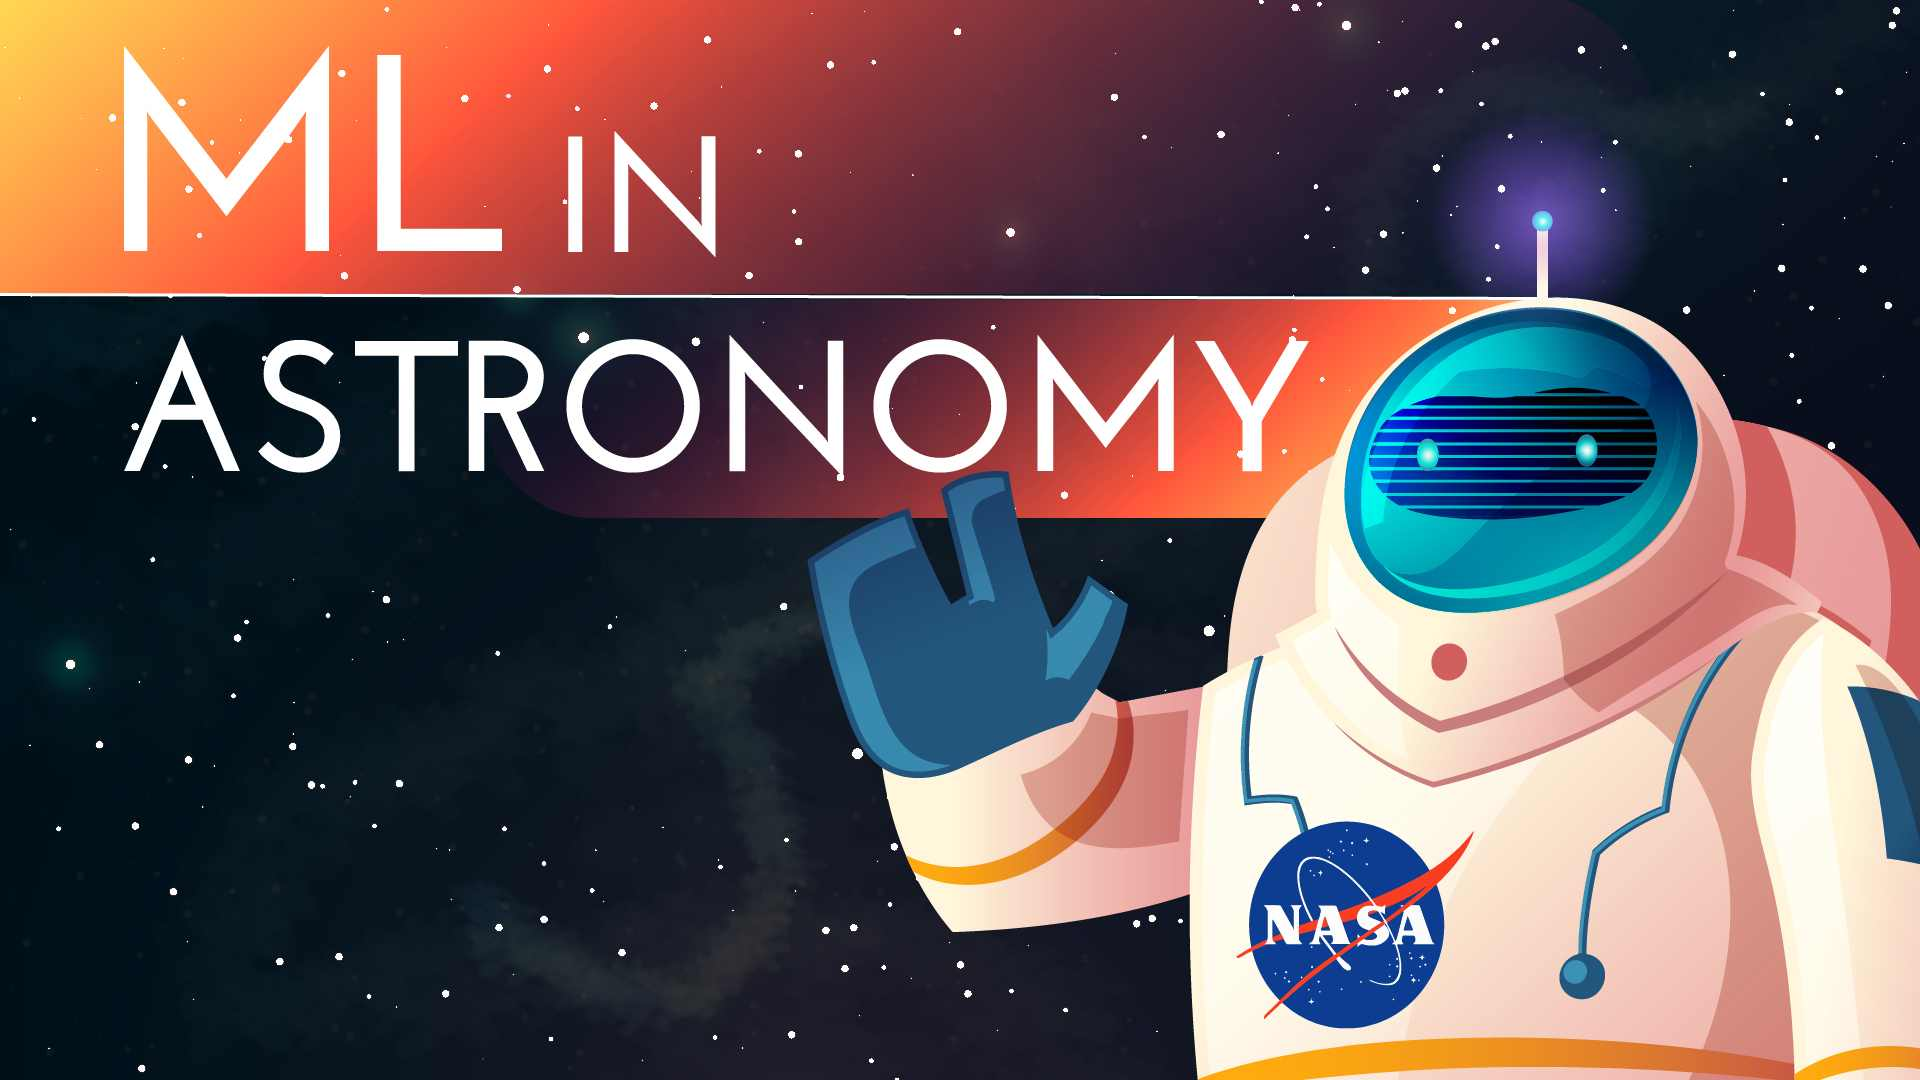
\includegraphics[height=6cm, angle=0,origin=c]{ml.jpg}
	
\end{frame}

	
\section{Questions}
\frame{
	\begin{itemize}
		\item What is \textbf{ML}?
		\item Why are we urged to implement \textbf{ML} in stronomy?
		\item What do we mean by \textbf{BIG DATA} in astronomy? 
		%\item What is the relation of \textbf{BIG DATA} and \textbf{ML} in astronomy? 
		\item Can \textbf{SKA} operate without \textbf{ML}?
		\item What are the limitations of \textbf{ML}?
	\end{itemize}
	}

\section{Machine Learning}\frame{text}
\subsection{a}\frame{}
\subsection{b}\frame{}
\section{Big Data}\frame{}
\subsection{a}\frame{}
\subsection{b}\frame{}
\section{SKA}\frame{text}
\subsection{a}\frame{}
\subsection{b}\frame{}
\section{Limitations}\frame{text}
\subsection{a}\frame{}
\subsection{b}\frame{}
\end{document}